\section{Convergence}

\subsection{Borel-Cantelli Lemmas}

  There are many Borel-Cantelli lemmas, and we will introduce the two most famous ones. To understand what these lemmas say, given a sequence $A_1, A_2, \ldots$ of events in $\sigma$-algebra $\mathcal{F}$, we must first understand what the daunting term  
  \begin{equation}
    \bigcap_{n=1}^\infty \bigcup_{i = n}^\infty A_i
  \end{equation}
  means. Now let's try to explain what the intersection of the unions mean. First, remember that $\sigma$-algebras are stable under both countable unions and countable intersections, this is also in $\mathcal{F}$. We can interpret 
  \begin{equation}
    \bigcap_{n=1}^\infty \bigcup_{i=n}^\infty A_i = \{ A_n \text{ i.o.}\}
  \end{equation}
  as the \textit{event that infinitely many $A_n$'s occur}, where i.o. means "infinitely often." To parse this, let's start from the innermost term and call it 
  \begin{equation}
    B_n = \bigcup_{i=n}^\infty A_i \implies \{A_n \text{ i.o.}\} = \bigcap_{n=1}^\infty B_n
  \end{equation}
  $B_n$ is the event that at least one of the $A_n, A_{n+1}, A_{n+2}, \ldots$ occurs, often referred to as the \textit{$n$th tail event}. Now the intersection of all $B_n$'s is the event that \textit{all} $B_n$'s occur. In other words, this is the event that for no matter how big of an $N \in \mathbb{N}$ I choose, there is always at least an event $A_n$ with $n > N$ that occurs. This is shortly summarized as the event that infinitely many $A_n$'s occur. 

  \begin{lemma}[1st Borel-Cantelli Lemma]
    Given probability space $(\Omega, \mathcal{F}, \mathbb{P})$, if $A_1, A_2, \ldots$ is a sequence of events such that 
    \begin{equation}
      \sum_{n=1}^\infty \mathbb{P}(A_n) < \infty
    \end{equation}
    the almost surely (with probability $1$) only finitely many $A_n$'s will occur. 
    \begin{equation}
      \mathbb{P} \bigg( \bigcap_{n=1}^\infty \bigcup_{i = n}^\infty A_i \bigg) = 0
    \end{equation}
  \end{lemma}
  \begin{proof}
    Setting $B_n$ as above, we have 
    \begin{align*}
      \mathbb{P}\bigg( \bigcap_{n=1}^\infty B_n \bigg) & = \lim_{n \rightarrow \infty} \mathbb{P}(B_n) & (\text{continuity of probability}) \\
      & = \lim_{n \rightarrow \infty} \mathbb{P} \bigg( \bigcup_{i=1}^\infty A_i \bigg) & (\text{substitute } B_i) \\
      & \leq \lim_{n \rightarrow \infty} \sum_{i = n}^\infty \mathbb{P}(A_i) = 0 & (\text{tail sum of convergent series is } 0)
    \end{align*}
  \end{proof}

  The second Borel-Cantelli lemma is like a partial contrapositive to the first lemma, where it starts with the assumption that the sum of the $\mathbb{P}(A_n)$'s are infinite (along with the addition case that they are independent). 

  \begin{lemma}[2nd Borel-Cantelli Lemma]
    If $A_1, A_2, \ldots$ are independent events such that 
    \begin{equation}
      \sum_{n=1}^\infty \mathbb{P}(A_n) = \infty,
    \end{equation}
    then almost surely (with probability $1$) infinitely many $A_n$'s will occur. That is, 
    \begin{equation}
      \mathbb{P} \bigg( \bigcap_{n=1}^\infty \bigcup_{i = n}^\infty A_i \bigg) = 1
    \end{equation}
  \end{lemma}

  The intuition behind this lemma is challenging: We can let $\mathbb{P}(A_n) = P_n$ and interpret the sum as a series of $P_n$'s. Since the series $P_1 + P_2 + \ldots$ is finite, this implies that 
  \begin{equation}
    \lim_{n \rightarrow \infty} P_n = 0
  \end{equation}
  (but not the converse) and going to zero rather fast such that the series is finite. So, you are working with a sequence of events $A_n$ that are becoming more and more unlikely rather fast. The lemma says that beyond a certain point $n_0$, none of the events $A_n$ will occur almost surely. For the second lemma, we can go as far as we like in the sequence of $A_n$'s, up to any $A_{n_0}$, but beyond that there is always an infinite number of $A_n$'s that occur beyond $A_{n_0}$. 

\subsection{Transforms}

  \subsubsection{Probability Generating Function (PGF)}

    The PGF is only defined for discrete random variable, and is analogous to the Z-transform in singal processing. 

    \begin{definition}[Probability Generating Function]
      Let $X$ be a discrete random variable taking values in $\mathbb{N}_0$. Then, the \textbf{probability generating function} of $X$ is defined 
      \begin{equation}
        G_X (z) \coloneqq \mathbb{E}[z^X] = \sum_{i=0}^\infty z^i \, \mathbb{P}(X = i)
      \end{equation}
      Now there is the problem of convergence, but we will not pay attention to this technicality for now and just consider the PGF as a tool. 
    \end{definition}

    \begin{example}[PGF of Poisson]
      The random variable $X \sim \mathrm{Poisson}(\lambda)$ has pmf $\mathbb{P}(X = i) = \frac{e^{-\lambda} \lambda^i}{i!}$ for $i \in \{0, 1, \ldots\}$. Then, 
      \begin{equation}
        G_X (z) = \mathbb{E}[z^X] = \sum_{i=0}^\infty z^i \, \frac{e^{-\lambda} \lambda^i}{i!} = \sum_{i=0}^\infty \frac{e^{-\lambda} (\lambda z)^i}{i!} = e^{\lambda(z - 1)}
      \end{equation}
    \end{example}

    \begin{example}[PGF of Geometric]
      For $X \sim \mathrm{Geometric}(p)$, its PGF is 
      \begin{equation}
        G_X (z) = \sum_{i=1}^\infty z^i \, (1 - p)^i p = \frac{p z}{1 - z(1 - p)}
      \end{equation}
    \end{example}

    \begin{lemma}[Properties of PGF]
      Given random variable $X$ and its PGF $G_X$, we have the following: 
      \begin{enumerate}
        \item Evaluate at $z = 1$: 
        \begin{equation}
          G_X (1) = \mathbb{E}[1^X] = \mathbb{E}[1] = 1
        \end{equation}
        \item Derivative at $z = 1$: 
        \begin{equation}
          \frac{d G_X (z)}{d z} \bigg|_{z = 1} = \mathbb{E}[X]
        \end{equation}
        \item $k$th derivative at $z = 1$: 
        \begin{equation}
          \frac{d^k G_X (z)}{d z^k} \bigg|_{z = 1} = \mathbb{E}[X (X-1) (X-2) \ldots (X-k +1)]
        \end{equation}
        \item Transformation: Given the sum $Z = X + Y$ (where $X, Y$ are independent), rather than computing its convolution, the PGF of $Z$ is simply the product of the PGFs of $X$ and $Y$: 
        \begin{equation}
          G_Z (z) = G_X (z) \, G_Y (z)
        \end{equation}
        For example, since a $\mathrm{Poisson}(\lambda)$ random variable has PGF of form $e^{\lambda (z - 1)}$, if we have two Poissons $X$ and $Y$ with parameters $\lambda, \mu$, then we can easily multiply their PGFs to get the PGF of $Z = X + Y$, which is $e^{(\lambda + \mu)(z - 1)}$, which is the PGF of a $\mathrm{Poisson}(\lambda + \mu)$ random variable. 
      \end{enumerate}
    \end{lemma}

  \subsubsection{Moment Generating Function (MGF)}

    \begin{definition}[Moment Generating Function (MGF)]
      The \textbf{moment generating function} associated with a random variable $X$ is a function $M_X: \mathbb{R} \longrightarrow [0, \infty]$ defined 
      \begin{equation}
        M_X (s) \coloneqq \mathbb{E}[e^{s X}]
      \end{equation}
      It is like an exponential moment. The region of convergence of $M_X$ is the set $D_X = \{s \mid M_X (s) < \infty\}$. 
      and we always have $M_X (0) = 1$, so $0 \in D_X$ always. 
    \end{definition}

    \begin{lemma}[Properties of MGF]
      Let $X$ be a random variable with MGF $M_X (s)$. 
      \begin{enumerate}
        \item $M_X (0) = 1$, so $0$ is always in the region of convergence. 
        \item If $Y = a X + b$, then 
        \begin{equation}
          M_Y (s) = e^{b s} M_X (a s)
        \end{equation}
        \item If $X$ and $Y$ are independent and $Z = X + Y$, then 
        \begin{equation}
          M_Z (s) = M_X (s) \, M_Y (s)
        \end{equation}
      \end{enumerate}
    \end{lemma}
    \begin{proof}
      Listed. 
      \begin{enumerate}
        \item $M_X (0) = \mathbb{E}[e^{0 X}] = \mathbb{E}[1] = 1$. 
        \item We have 
        \begin{align*}
          M_Y (s) & = \mathbb{E} [e^{s(a X + b)}] \\
          & = \mathbb{E}[ e^{a s X } e^{b s}] \\
          & = \mathbb{E}[e^{(as) X}] \, \mathbb{E}[e^{b s}] \\
          & = e^{b s} M_X (a s)
        \end{align*}
        where the penultimate step was due to independence of constant RV with any other RVs. 
        \item We can see 
        \begin{equation}
          M_Z (s) = \mathbb{E}[ e^{s (X + Y)}] = \mathbb{E}[e^{s X} \, e^{s Y}] = \mathbb{E}[e^{s X}] \, \mathbb{E}[e^{s Y}] = M_X (s) \, M_Y (s)
        \end{equation}
        since $X, Y$ independent means that any function of $X$ and $Y$ are independent. 
      \end{enumerate}
    \end{proof}

    \begin{theorem}[Inversion Theorem]
      Suppose $M_X (s)$ is finite for all $s \in [-\epsilon, \epsilon]$ for some $\epsilon > 0$. Then, $M_X$ uniquely determines the CDF of $X$. This implies that if $X$ and $Y$ are random variables such that $M_X (s) = M_Y (s)$ for all $s \in [-\epsilon, \epsilon]$ for some $\epsilon > 0$, then $X$ and $Y$ have the same CDF. 
    \end{theorem}

    This theorem is useful for comparing random variables with the MGFs, but a limitation is that it is not always clear that the MGF is defined beyond $0$. Now, we explain why this is called a moment generating function. 

    \begin{theorem}[Moment Generating Property]
      Suppose $M_X (s) < \infty$ for $s \in [-\epsilon, \epsilon]$ with $\epsilon > 0$. Then, the derivatives at $s = 0$ generate the moments of $X$: 
      \begin{equation}
        \frac{d^m M_X (s)}{d s^m} \bigg|_{s = 0} = \mathbb{E}[X^m]
      \end{equation}
    \end{theorem}
    \begin{proof}
      A hand-wavy proof is that we can take the derivative and put it "in" the expectation. 
      \begin{equation}
        \frac{d}{ds} \mathbb{E}[e^{s X}] = \mathbb{E} \big[ \frac{d}{ds} e^{s X} \big] = \mathbb{E}[X e^{s X}]
      \end{equation}
      which evaluates to $\mathbb{E}[X]$ when $s = 0$. Differentiating $m$ times just gets $\mathbb{E}[X^m e^{s X}]$. However, this should be questioned, since the expectation is an integral and we are putting the derivative inside the integral. 
    \end{proof}

    \begin{example}[Exponential RV]
      The PDF of $X \sim \mathrm{Exponential}(\mu)$ is $f_X (x) = \mu e^{-\mu x}$ for $x \geq 0$. The MGF is 
      \begin{equation}
        M_X (s) \coloneqq \int_0^\infty \mu e^{-\mu x} e^{s x} \, dx = \begin{cases} 
        \frac{\mu}{\mu - s} & \text{ for } s < \mu \\
        \infty & \text{ for } s \geq \mu 
      \end{cases}
      \end{equation}
    \end{example}

    \begin{example}[Gaussian RV]
      The PDF of a standard Gaussian $X$ is $f_X (x) = \frac{1}{\sqrt{2\pi}} e^{-x^2 / 2}$ for $x \in \mathbb{R}$, and the MGF is 
      \begin{equation}
        M_X (s) = \int_{-\infty}^\infty \frac{1}{\sqrt{2 \pi}} e^{- x^2 / 2} e^{s x} \,dx = e^{s^2 / 2} \int_{-\infty}^\infty \frac{1}{\sqrt{2\pi}} e^{-\frac{(x - s)^2}{2}}\,dx = e^{s^2 / 2}
      \end{equation}
      which is valid for all $s \in \mathbb{R}$. 
    \end{example}

    \begin{example}[Cauchy RV]
      If we have $f_X (x) = \frac{1}{\pi} \frac{1}{1 + x^2}$ for $x \in \mathbb{R}$, the MGF is 
      \begin{equation}
        M_X (s) = \int_{-\infty}^\infty \frac{e^{s x}}{\pi (1 + x^2)} \,dx = \begin{cases} 1 & \text{ if } s = 0 \\
        \infty & \text{ if } s > 0 \\ 
        \infty & \text{ if } s < 0 \end{cases}
      \end{equation}
      So the region of convergence is just $\{0\}$. It is infinity everywhere else since the exponential function grows exponentially as $x \rightarrow \pm \infty$. 
    \end{example}

    \begin{example}
      Given $X_1 \sim \mathrm{Exponential}(\lambda_1)$ and $X_2 \sim \mathrm{Exponential}(\lambda_2)$ are independent, the MGF of $Z = X_1 + X_2$ is 
      \begin{equation}
        M_Z (s) = M_X (s) \, M_Y (s) = \frac{\lambda_1 \lambda_2}{(\lambda_1 - s)(\lambda_2 - s)} \text{ for } s < \min\{\lambda_1, \lambda_2\}
      \end{equation}
      and we can perform our inverse transform on it. 
    \end{example}

  \subsubsection{Characteristic Function}

    We can see that the MGF has its limitations: for some random variables (like the Cauchy), its MGF was not defined at all beyond $\{0\}$. On the contrary, the characteristic function is always defined everywhere and is finite everywhere (in fact, is bounded by $1$, shown below). Also, it is a bit easier to invert (similar to how the Fourier transform is a bit easier to invert than the Laplace). 

    \begin{definition}[Characteristic Function]
      Given a random variable $X: \Omega \longrightarrow \mathbb{R}$, the \textbf{characteristic function} is defined to be 
      \begin{align*}
        \varphi_X (t) & = \mathbb{E}[ e^{i t X} ] \\
        & = \mathbb{E}[\cos{(t X)}] + i \mathbb{E}[ \sin{(t X)}]
      \end{align*}
    \end{definition}

    If $X$ admits a PDF, then the characteristic function is its Fourier transform with a small sign reversal. 
    \begin{equation}
      \varphi_X (t) = \int_\mathbb{R} e^{i t x} f_X (x)\,dx
    \end{equation}

    \begin{theorem}[Properties of CF]
      Let $X$ be a random variable with CF $\varphi_X (t)$. 
      \begin{enumerate}
        \item $\varphi_X (0) = 1$  and $|\varphi_X (t)| \leq 1$ for all $t \in \mathbb{R}$. 
        \item If $Y = a X + b$, then 
        \begin{equation}
          \varphi_Y (t) = e^{i b t} \varphi_X (a t)
        \end{equation}
        \item If $X$ and $Y$ are independent random variables and $Z = X + Y$, then 
        \begin{equation}
          \varphi_Z (t) = \varphi_X (t) \, \varphi_Y (t)
        \end{equation}
        \item $\varphi_X (t)$ is uniformly continuous on $\mathbb{R}$, i.e. for all $t \in \mathbb{R}$, there exists a $\phi(h) \downarrow 0$ as $h \downarrow 0$ such that 
        \begin{equation}
          |\varphi_X (t + h) - \varphi_X (t)| \leq \phi(h)
        \end{equation}
        \item $\varphi_X$ is a nonnegative-definite kernel, i.e. for any $n$ reals $t_1, \ldots, t_n$ and $n$ complex numbers $z_1, \ldots z_n$, we have 
        \begin{equation}
          \sum_{i, j} z_i \varphi_X (t_i - t_j) \, \bar{z}_j \geq 0
        \end{equation}
      \end{enumerate}
    \end{theorem}
    \begin{proof}
      Listed. 
      \begin{enumerate}
        \item We just set $\varphi_X (0) = \mathbb{E}[e^{i 0 X}] = \mathbb{E}[1] = 1$, and for continuous random variables, we can bound 
        \begin{align*}
          \big| \varphi_X (t) \big| & = \bigg| \int_{-\infty}^\infty e^{i t x} f_X (x) \,dx  \bigg| \\
          & \leq \int_{-\infty}^\infty \big| e^{i t x} f_X (x) \big| \,dx \\
          & \leq \int_{-\infty}^\infty \big| e^{i t x} \big| \cdot \big|f_X (x) \big| \,dx \\
          & = \int_{-\infty}^\infty f_X (x) \,dx = 1 
        \end{align*}
        
        \item We have 
        \begin{equation}
          \varphi_Y (t) = \mathbb{E}[ e^{i t (a X + b)}] = \mathbb{E}[ e^{i a t X} \, e^{i b t}] = \mathbb{E}[ e^{i (at) X}] \, \mathbb{E}[e^{i b t}] = e^{i b t} \varphi_X (a t)
        \end{equation}
        
        \item We have 
        \begin{equation}
          \varphi_Z (t) = \mathbb{E}[ e^{i t (X + Y)}] = \mathbb{E}[ e^{i t X} \, e^{i t Y}] = \mathbb{E}[e^{i t X}] \, \mathbb{E}[e^{i t Y}] = \varphi_X (t) \, \varphi_Y (t)
        \end{equation}
        
        \item We have 
        \begin{align*}
          | \varphi_X (t + h) - \varphi_X (t)| & = | \mathbb{E} [ e^{i tX} (e^{i h X} - 1)] | \\ 
          & \leq \mathbb{E}[ | e^{i tX} (e^{i h X} - 1)|] \\
          & \leq \mathbb{E}[ |e^{i h X} - 1|] \ldots
        \end{align*}
      \end{enumerate}
    \end{proof}

    Now this next theorem states the uniqueness of each characteristic function. It is a highly nontrivial result. 

    \begin{theorem}[Inversion Theorem]
      If two random variables have the same characteristic function, then their CDFs are the same. Further, if $X$ is a continuous random variable, then the PDF can be recovered from the characteristic function as follows: 
      \begin{equation}
        f_X (x) = \lim_{T \rightarrow \infty} \frac{1}{2 \pi} \int_{-T}^T e^{- i t x} \varphi_X (t) \,dt
      \end{equation}
      for every $x$ where $f_X (x)$ is continuous. 
    \end{theorem}

    Just like how we can recover moments from the MGF, we can always recover the moments from the characteristic function, with the added advantage that the CF will always exist. 

    \begin{theorem}[Moment Generating Property]
      Let $X$ be a random variable and $\varphi_X (t)$ its CF. 
      \begin{enumerate}
        \item If $\varphi_X^{(k)} (t)$ ( the $k$th derivative) exists at $t = 0$, then 
        \begin{align*}
          \mathbb{E}[|X^k|] < \infty & \text{ for } k \text{ even} \\
          \mathbb{E}[|X^{k-1}|] < \infty & \text{ for } k \text{ odd}
        \end{align*}
        
        \item If $\mathbb{E}[|X^k|] < \infty$, then 
        \begin{equation}
          \varphi_X^{(k)} (0) = i^k \mathbb{E}[X^k]
        \end{equation}
        
        \item Further, given that the moments are finite, we can expand the CF by moments of $X$ as 
        \begin{equation}
          \varphi_X (t) = \sum_{j=0}^k \frac{\mathbb{E}[X^j]}{j!} (i t)^j + o(t^k)
        \end{equation}
      \end{enumerate}
    \end{theorem}

    \begin{example}[Bernoulli]
      Given $X \sim \mathrm{Bernoulli}(p)$, we have 
      \begin{align*}
        \mathbb{E}[ e^{i t X}] & = \sum_{x \in \{0, 1\}} e^{i t x} \cdot \mathbb{P}(X = x) \\
        & = e^{i t 0} (1 - p) + e^{i t} p \\
        & = 1 - p + p e^{i t}
      \end{align*}
    \end{example}

    \begin{example}[Exponential]
      Given $X \in \mathrm{Exponential}(\lambda)$, we have 
      \begin{align*}
        \mathbb{E}[e^{i t X}] & = \int_0^\infty e^{i t x} \lambda e^{-\lambda x} \,dx \\
        & = \int_0^\infty \lambda \, e^{-(\lambda - i t) x} \,dx \\
        & = \frac{\lambda}{\lambda - it} \text{ for all } t \in \mathbb{R}
      \end{align*}
      where the complex integral requires some complex analysis. 
    \end{example}

\subsection{Convergence of Random Variables}

  Unlike convergence of numbers, which is well-defined with respect to some metric or topology, there are many types of convergence of random variables. We must always specify which convergence when talking about them. Remember that a random variable $X$ is just a function from $\Omega$ to $\mathbb{R}$, so we can talk about pointwise convergence. That is, given a sequence of random variables $\{X_n\}$ and some $\omega \in \Omega$, the sequence 
  \begin{equation}
    X_1(\omega), X_2 (\omega), X_3(\omega), \ldots
  \end{equation}
  is simply a sequence of real numbers. If this sequence converges to the real number $X(\omega)$, then $X_n$ converges to $X$ at $\omega$. If this occurs for all $\omega \in \Omega$, then we have sure convergence, and if this happens for an event (a $\mathcal{F}$-measurable subset of $\Omega$) with probability $1$, then we have almost sure convergence. 

  \begin{definition}[Sure Convergence of RVs]
    The sequence of random variables $\{ X_n\}_{n \in \mathbb{N}}$ is said to \textbf{converge pointwise} or \textbf{converge surely} to $X$ if 
    \begin{equation}
      X_n (\omega) \rightarrow X (\omega)
    \end{equation}
    for every $\omega \in \Omega$. That is, we can choose \textit{any} $\omega \in \Omega$, and the realized sequence $X_1 (\omega), X_2 (\omega), \ldots$ will always converge to $X(\omega)$. We can visualize the function $X$ with a surface defined over $\Omega$ and can imagine the $X_n$'s as surfaces that converges to that of $X$. 
    \begin{center}
      \includegraphics[scale=0.3]{img/sure_convergence.jpg}
    \end{center}
  \end{definition}

  But this definition is too strong of a form of convergence, since in probability we don't care about values over sets of measure $0$. That is, if we have two probability distributions that differ from each other on a set of measure $0$, then they can be considered essentially the same probability distribution. 

  \begin{definition}[Almost Sure Convergence of RVs]
    The sequence of random variables $\{ X_n\}_{n \in \mathbb{N}}$ is said to \textbf{converge almost surely} or \textbf{converge with probability 1} to $X$ if $X_n (\omega) \rightarrow X (\omega)$ on a subset of probability $1$. That is, 
    \begin{equation}
      \mathbb{P} \big( \{ \omega \in \Omega \mid \lim_{n \rightarrow \infty} X_n (\omega) = X(\omega) \} \big) = 1
    \end{equation}
    Considering small technicalities, it can be shown that this set of $\omega$'s can be considered an event in $\mathcal{F}$. This can be visualized similarly as sure convergence, but now the surfaces don't have to converge on sets of measure $0$. 
    \begin{center}
      \includegraphics[scale=0.3]{img/almost_sure_convergence.jpg}
    \end{center}
    Crudely put, we just have to look at each $\omega \in \Omega$, see if $X_n (\omega)$ converges to $X(\omega)$ as $n \rightarrow \infty$, and determine if the set of all $\omega$'s that satisfy this have probability $1$. In other words, let us have some experiment with outcome space $\Omega$. With probability $1$, some $\omega \in \Omega$ will be realized, which will realize the sequence of realized random variables
    \begin{equation}
      X_1 (\omega), X_2 (\omega), X_3 (\omega), \ldots
    \end{equation}
    that will converge to $X(\omega)$. Visually, we can imagine selecting a random point in $\Omega$, which will not hit the curve or point (with probability $1$), and in these cases, the sequence of points will converge to $X(\omega)$. 
    \begin{center}
      \includegraphics[scale=0.3]{img/almost_sure_convergence_2.jpg}
    \end{center}
  \end{definition}

  \begin{definition}[Convergence in Probability]
    The sequence of random variables $\{ X_i\}_{i \in \mathbb{N}}$ is said to \textbf{converge to $X$ in probability} if for all $\epsilon > 0$, 
    \begin{equation}
      \lim_{n \rightarrow \infty} \mathbb{P} \big( |X_n - X| > \epsilon \big) = 0
    \end{equation}
    To understand what this means, fix an $\epsilon > 0$. Then, $X_1$ may be very far from $X$, meaning that the event $|X_1 - X| > \epsilon$, i.e. the set of all $\omega \in \Omega$ satisfying $|X_1(\omega) - X (\omega)| > \epsilon$ may be a larger portion of $\Omega$. Now, as we increase $n$, this event will become smaller (in the way that it's probability decreases) until it reaches $0$. 
    \begin{center}
      \includegraphics[scale=0.3]{img/convergence_in_probability.jpg}
    \end{center}
  \end{definition}

  \begin{example}
    Given $X_n \sim \mathrm{Exponential}(n)$ with $f_{X_n} (x) = n e^{-nx}$, we show that the sequence converges in probability to the $0$ random variable. Given $\epsilon > 0$, we have 
    \begin{align*}
      \lim_{n \rightarrow \infty} \mathbb{P}(|X_n - 0| > \epsilon) & = \lim_{n \rightarrow \infty} \mathbb{P}(X_n > \epsilon \cup X_n < -\epsilon) \\
      & = \lim_{n \rightarrow \infty} \mathbb{P}(X_n > \epsilon) \\
      & = \lim_{n \rightarrow \infty} \int_\epsilon^\infty n e^{-nx} \,dx \\
      & = \lim_{n \rightarrow \infty} e^{-n \epsilon} = 0
    \end{align*}
    We can imagine this since given any small $\epsilon > 0$, we can see that increasing $n$ results in the distribution of $X_n$ to decrease at a faster rate, and thus a bigger portion of the distribution would lie within $\epsilon$ of the $0$ random variable. 
    \begin{center}
      \includegraphics[scale=0.3]{img/convergence_in_prob_exponential.jpg}
    \end{center}
  \end{example}

  \begin{definition}[Convergence in rth Mean]
    We say $X_n$ \textbf{converges to $X$ in the $r$th mean} if 
    \begin{equation}
      \lim_{n \rightarrow \infty} \mathbb{E} \big[ |X_n - X|^r \big] = 0
    \end{equation}
    For $r = 2$, $X_n$ is said to converge to $X$ in the \textbf{mean-squared sense}. 
  \end{definition}

  \begin{definition}[Convergence in Distribution]
    We say $X_n$ \textbf{converges to $X$ in distribution} if the CDF of $X_n$ converges pointwise to the CDF of $X$, i.e. 
    \begin{equation}
      \lim_{n \rightarrow \infty} F_{X_n} (x) = F_X (x)
    \end{equation}
    for all $x$ where $F_{X}$ is continuous. 
  \end{definition}

  So for practical purposes there are 5 notions of convergence that we will work with: 
  \begin{enumerate}
      \item Sure convergence: $X_n \xrightarrow{p.w.} X$ 
      \item Almost sure convergence: $X_n \xrightarrow{a.s.} X$ 
      \item Convergence in probability: $X_n \xrightarrow{i.p.} X$ 
      \item Convergence in $r$th mean: $X_n \xrightarrow{rth} X$ (Mean square: $X_n \xrightarrow{m.s.} X$) 
      \item Convergence in distribution: $X_n \xrightarrow{D} X$
  \end{enumerate}

  \begin{theorem}[Hierarchy of Convergence]
    The following implications hold: 
    \begin{enumerate}
      \item Pointwise c. $\implies$ almost sure c. $\implies$ c. in probability $\implies$ c. in distribution. 
      \item $r$th mean c. $\implies$ c. in probability $\implies$ c. in distribution. 
    \end{enumerate}
  \end{theorem}

  Trying to understand these relationships can be very hard, so we will take some time to do that, with some examples. First, convergence in distribution is clearly the weakest, since convergence in distribution does not imply that the random variables need be close to each other. Take a look at the random variables $X \sim \mathrm{Bernoulli}(1/2)$ and $Y = 1 - X$. $X$ and $Y$ are both $\mathrm{Bernoulli}(1/2)$ with the same distribution, but they are \textit{not} the same random variable since $X - Y = 1$ always. Therefore, we can think of two random variables that have the same distribution but are not "close" to each other as functions over $\Omega$ that divide it into identical, but differently cut, distributions. 

  \begin{figure}[H]
    \centering 
    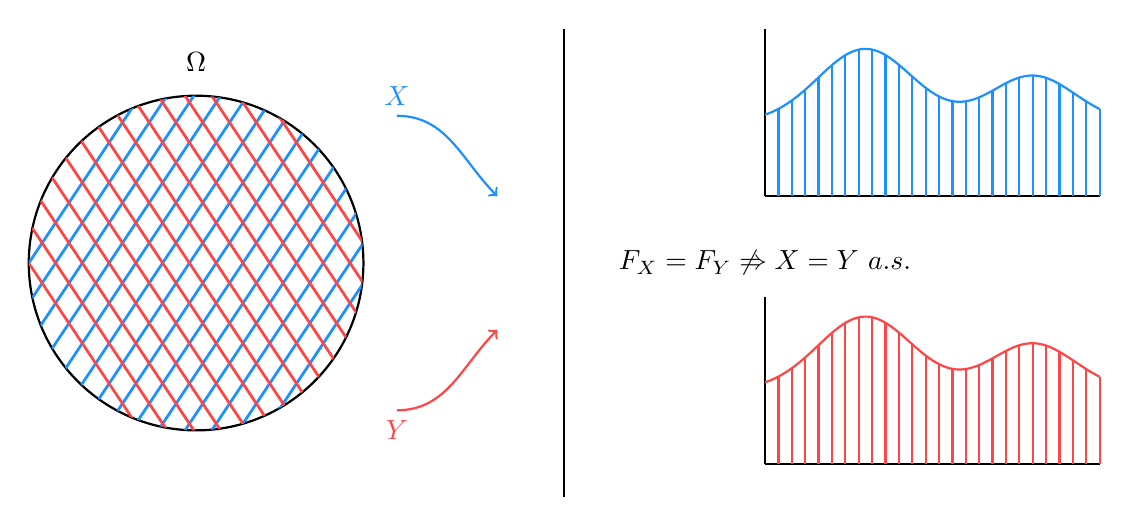
\begin{tikzpicture}[scale=0.85]
      % Define colors
      \definecolor{xcolor}{RGB}{30,144,255}  % Blue
      \definecolor{ycolor}{RGB}{255,70,70}   % Red
      
      % Load patterns library
      \usetikzlibrary{patterns}
      
      % Probability space (Omega)
      \begin{scope}
        \node at (-3.5,3) {$\Omega$};
        \draw[thick] (-3.5,0) circle (2.5);
        
        % Create custom patterns with proper colors and denser lines
        \begin{scope}
          % Blue lines pattern (X) - with reduced spacing between lines
          \clip (-3.5,0) circle (2.5);
          \foreach \i in {-8,-7.6,-7.2,...,5} {
            \draw[xcolor, line width=1.0pt] (\i,-3) -- (\i+4,3);
          }
        \end{scope}
        
        \begin{scope}
          % Red lines pattern (Y) - with reduced spacing between lines
          \clip (-3.5,0) circle (2.5);
          \foreach \i in {-8,-7.6,-7.2,...,2} {
            \draw[ycolor, line width=1.0pt] (\i+4,-3) -- (\i,3);
          }
        \end{scope}
      \end{scope}
      
      % X random variable label and arrow
      \node[xcolor] at (-0.5,2.5) {$X$};
      \draw[->, xcolor, thick, out=0, in=135] (-0.5,2.2) to (1,1);
      
      % Y random variable label and arrow
      \node[ycolor] at (-0.5,-2.5) {$Y$};
      \draw[->, ycolor, thick, out=0, in=225] (-0.5,-2.2) to (1,-1);
      
      % Vertical dividing line
      \draw[thick] (2,-3.5) -- (2,3.5);
      
      % Define distribution function once to ensure consistency
      \pgfmathdeclarefunction{distfunc}{1}{%
        \pgfmathparse{0.1+1.1*exp(-(#1-1.5)^2/1.0)+0.7*exp(-(#1-4)^2/0.8)}%
      }
      
      % X distribution (top right)
      \begin{scope}[shift={(5,2)}]
        \draw[thick] (0,-1) -- (5,-1);
        \draw[thick] (0,-1) -- (0,1.5);
        
        % Calculate curve points directly from the function to ensure alignment
        \draw[xcolor, thick] plot[smooth, domain=0:5, samples=50] 
          (\x, {distfunc(\x)});
        
        % Vertical lines for X distribution
        \foreach \i in {0.2,0.4,...,5} {
          \pgfmathsetmacro{\yval}{distfunc(\i)}
          \draw[xcolor, line width=0.8pt] (\i,-1) -- (\i,\yval);
        }
      \end{scope}
      
      % Relationship text
      \node at (5,0) {$F_X = F_Y \not\Rightarrow X=Y\ a.s.$};
      
      % Y distribution (bottom right)
      \begin{scope}[shift={(5,-2)}]
        \draw[thick] (0,-1) -- (5,-1);
        \draw[thick] (0,-1) -- (0,1.5);
        
        % Calculate curve points directly from the function to ensure alignment
        \draw[ycolor, thick] plot[smooth, domain=0:5, samples=50] 
          (\x, {distfunc(\x)});
        
        % Vertical lines for Y distribution
        \foreach \i in {0.2,0.4,...,5} {
          \pgfmathsetmacro{\yval}{distfunc(\i)}
          \draw[ycolor, line width=0.8pt] (\i,-1) -- (\i,\yval);
        }
      \end{scope}
    \end{tikzpicture}
    \caption{Two identical distributions may not model the same phenomenon.} 
    \label{fig:prob_in_dist}
  \end{figure}

  \begin{example}[C. in Distribution $\centernot\implies$ C. in Probability]
    Let $X_1, X_2, \ldots$ be such that $X_i = X$ for all $i$ where $X \sim \mathrm{Bernoulli}(1/2)$. This does not mean that the $X_i$'s are iid Bernoulli; they are all copies of the same $X$, i.e. forms a constant sequence. Let $Y = 1 - X$. Clearly, $X_n \xrightarrow{D} Y$ since the CDF of every $X_i$ is the same as that of $Y$, but $|X_n - Y| = 1$ for all $n$, so there is no convergence.  
  \end{example}

  \begin{example}[C. in Distribution $\centernot\implies$ C. in Probability]
    Let $X_1, X_2, \ldots \sim \mathcal{N}(0, 1)$ and $Y = -X$. Then, by symmetry of the standard Gaussian, both $X$ and $Y$ have the same CDF, but they are not the same random variable: their signs are opposite. 
  \end{example}

  \subsubsection{Convergence in Probability vs Almost Surely} 

    Convergence almost surely and convergence with probability are very different. Almost sure convergence has the limit inside the probability, which indicates that we are talking about convergence of a sequence of random variables. On the other hand, convergence in probability has the limit on the outside, which talks about convergence of a sequence of probabilities. But a key point is that almost sure convergence implies convergence in probability. It happens so because there could exist a subset of small probability in $\Omega$ where the $X_n$'s and $X$ need not be close, but the probabilities of them deviating over whole $\Omega$ is small. 

    \begin{example}[C. in Probability $\centernot\implies$ C. Almost Surely]
      Consider the interval $\Omega = [0, 1]$ and the subsets $A_1 = [0, 0.1], A_2 = [0.1, 0.2], \ldots$, such that at $A_{10} = [0.9, 1.0]$, the size with halve and will go to the left boundary, $A_{11} = [0, 0.05], \ldots$. Then, the sequence of indicator random variables 
      \begin{equation}
        X_n \coloneqq 1_{A_n}
      \end{equation}
      looks like it's converging to the $0$ random variable. Indeed, $X_n \xrightarrow{i.p.} 0$ since the probability that $X_n$ deviates from $0$ by more than some small $\epsilon$ is simply the measure of $A_n$ itself, which decreases to $0$. That is, given some small $\epsilon > 0$, we have 
      \begin{equation}
        \lim_{n \rightarrow \infty} \mathbb{P} (|X_n - 0| > \epsilon) = \lim_{n \rightarrow \infty} \mathbb{P}(1_{A_n} > \epsilon ) = \lim_{n \rightarrow \infty} \mathbb{P}(A_n) = 0
      \end{equation}
      Now let's show that this doesn't converge almost surely. For \textit{any} outcome $\omega \in \Omega$, the sequence of random variables $X_1(\omega), X_2(\omega), \ldots$ will hit these intervals $A_n$ infinitely many times and will not converge to $0$, since there will always be a $1$ down the sequence. They will occur with decreasing frequency but they will always occur. Therefore, with probability $1$, whatever realized sequence will not converge to the $0$ random variable. 
    \end{example}

    Here is another standard counterexample. 

    \begin{example}[C. in Probability $\centernot\implies$ C. Almost Surely]
      Let us take the sequence $X_1, X_2, \ldots$ of independent random variables where $X_n \sim \mathrm{Bernoulli}(1/n)$. That is, 
      \begin{equation}
        \mathbb{P}(X_n = 1) = \frac{1}{n} \text{ and } \mathbb{P}(X_n = 0) = 1 - \frac{1}{n}
      \end{equation}
      So, as $n$ gets large we expect $X_n$ to realize values of $0$ more and more. Showing that $X_n \xrightarrow{i.p.} 0$ is easy, since we can compute for any $\epsilon > 0$
      \begin{align*}
        \lim_{n \rightarrow \infty} \mathbb{P}(|X_n - 0| > \epsilon) & = \lim_{n \rightarrow \infty} \mathbb{P}(|X_n| > \epsilon) \\
        & = \lim_{n \rightarrow \infty} \mathbb{P}(X_n = 1) \\
        & = \lim_{n \rightarrow \infty} \frac{1}{n} = 0
      \end{align*}
      We want to show that this does not converge almost surely to $0$, i.e. there is some set of nonzero measure such that for some $\omega$ in that set, the sequence $X_1 (\omega), X_2(\omega), \ldots$ does not converge to $0$. This can be hard to see at first, but the fact that we have independence and the terms are $\frac{1}{n}$ hints at the Borel-Cantelli lemma. Let $A_n$ be the event that $\{X_n = 1\}$ (i.e. the preimage of the singleton set under $X_n$: $X_n^{-1} ( \{1\})$). Then, the $A_n$'s are independent, and 
      \begin{equation}
        \sum_{n=1}^\infty \mathbb{P}(A_n) = +\infty
      \end{equation}
      By the Borel-Cantelli lemma 2, this implies that almost surely infinitely many $A_n$'s will occur. That is, we can choose as large of an $n$ as we like, go down the sequence until we look at $X_n, X_{n+1}, \ldots$, and we are guaranteed with probability $1$ that at least one of the $X_i$'s after $n$ will realize a $1$. This means that in every realization of $X_1, X_2, \ldots$, we will get a sequence of $0$s and $1$s, but since BCL states that no matter how far down the road you will always get at least another $1$, this sequence does not converge to $0$.  
    \end{example}

    The commonality between these two examples is that sequence of random variables satisfies convergence in probability as follows: As $n$ increases, $X_n$ is more and more likely to be near $X$ (in the way that $|X_n - X| < \epsilon$ for some $\epsilon > 0$), ultimately satisfying this closeness property with probability $1$ as $n \rightarrow \infty$. For example, we could have 
    \begin{align*}
      \mathbb{P}(|X_1 - X| > \epsilon) & = 1 \\
      \mathbb{P}(|X_2 - X| > \epsilon) & = 1/2 \\
      \mathbb{P}(|X_3 - X| > \epsilon) & = 1/3 \\
      \ldots & = \ldots 
    \end{align*}
    This definitely satisfies convergence in probability, but this leaves open the possibility that $\mathbb{P}(|X_n - X| > \epsilon)$ an infinite number of times, although at infrequent intervals. Therefore, when looking at the sequence 
    \begin{equation}
      X_1, X_2, X_3, \ldots
    \end{equation}
    each random variable \textit{individually} may have less chance of being more than $\epsilon$ away from $X$, but since there is an infinite number of them in the sequence, the sequence \textit{in totality} may contain an infinite number of cases where $|X_n - X| > \epsilon$. Convergence almost surely tells us that we are \textit{guaranteed} (with probability $1$) that this sequence will converge to $X$. That is, we can specify an $N \in \mathbb{N}$ such that $|X_n - X| < \epsilon$ for all $n > N$. 

    Let us define some $\epsilon > 0$ and consider a sequence of random variables $\{X_n\}_{n \in \mathbb{N}}$. Given some outcome $\omega \in \Omega$, we will consider it a \textit{success} if $|X_n(\omega) - X(\omega)| < \epsilon$ and \textit{failure} if not. Then, convergence in probability tells us that the probability of failure goes to $0$ as $n$ goes to infinity and therefore we get better and better estimates of $X$. Convergence almost surely is a bit stronger and says that the total number of failures is \textit{finite}. That is, after a certain point $N$, the random variable $X_n$ will \textit{always} estimate $X$ within an error of $\epsilon$ (i.e. such that $|X_n - X| < \epsilon$). But since you don't know when you've exhausted all failures, there is not much of a difference from a practical point of view. 

  \subsubsection{Complete Convergence}

    When proving almost sure convergence, we'd ideally just look at all the $\omega \in \Omega$ where $X_n (\omega) \rightarrow X(\omega)$, and if this set has probability measure $1$, then we are done. But this is not very practical, so we use the following theorem, which gives a sufficient condition for $X_n \xrightarrow{a.s.} X$. 

    \begin{theorem}
      If for all $\epsilon > 0$, 
      \begin{equation}
        \sum_{n=1}^\infty \mathbb{P}(|X_n - X| > \epsilon ) < \infty
      \end{equation}
      then $X_n \xrightarrow{a.s.} X$. This condition is a bit stronger, since not only are we saying that $\mathbb{P}(|X_n - X| > \epsilon)$ tends to $0$ as $n \rightarrow \infty$, but that it goes down fast enough to keep the series convergent. 
    \end{theorem}
    \begin{proof}
      Let the event that $|X_n - X| > \epsilon$ be denoted $A_n (\epsilon)$ (i.e. the preimage of $(\epsilon, \infty)$ under the map $|X_n - X|$, which is a $\mathcal{F}$-measurable set). Since the sum of their probabilities is finite, by the Borel-Cantelli lemma 1, finitely many $A_n(\epsilon)$'s will occur with probability $1$. This means that for any $\epsilon > 0$, $|X_n - X| \leq \epsilon$ for all large enough $n$, meaning that it converges to $0$. 
    \end{proof}

\subsection{Laws of Large Numbers}

  \begin{theorem}[Weak Law of Large Numbers]
    Let $X_1, X_2, ..., X_n$ be a sequence of iid random variables, with finite mean $\mathbb{E}[X]$. Then, the average of the random variables $S_n / n$ converges in probability to $\mathbb{E}[X]$. 
    \begin{equation}
      \frac{S_n}{n} = \frac{1}{n} \sum_{i=1}^n X_i \xrightarrow{i.p} \mathbb{E}[X]
    \end{equation}
    That is, for any $\epsilon > 0$, 
    \begin{equation}
      \lim_{n \rightarrow \infty} \mathbb{P} \bigg( \bigg| \Big( \frac{1}{n} \sum_{k=1}^n X_k \Big) - \mathbb{E}[X] \bigg| > \epsilon \bigg) = 0
    \end{equation}
  \end{theorem}
  \begin{proof}
    We first do the proof assuming additionally that $X$ has finite variance, so $\mathrm{Var}[X] < \infty$. We will show that the random variable $S_n/n$ converges in mean square to $\mathbb{E}[X]$, which will imply convergence in probability. Note that $\mathbb{E}[S_n / n] = \mathbb{E}[X]$, and 
    \begin{align*}
      \lim_{n \rightarrow \infty} \mathbb{E} \bigg[ \bigg| \frac{S_n}{n} - \mathbb{E}[X] \bigg|^2 \bigg] & = \lim_{n \rightarrow \infty} \mathbb{E} \bigg[ \bigg| \frac{S_n}{n} - \mathbb{E}\Big[\frac{S_n}{n}\Big] \bigg|^2 \bigg] \\
      & = \lim_{n \rightarrow \infty} \mathrm{Var}\Big( \frac{S_n}{n} \Big) \\
      & = \lim_{n \rightarrow \infty} \frac{\mathrm{Var}(S_n)}{n^2} \\
      & = \lim_{n \rightarrow \infty} \frac{\mathrm{Var}[X]}{n} = 0
    \end{align*}
  \end{proof}

  \begin{theorem}[Strong Law of Large Numbers]
    Let $X_1, X_2, ..., X_n$ be a sequence of iid random variables, with finite mean $\mathbb{E}(X_k)$ and with finite variance. Then, the average of the random variables $S_n / n$ converges almost surely to $\mathbb{E}[X]$. 
    \begin{equation}
      \frac{S_n}{n} \xrightarrow{a.s.} \mathbb{E}[X]
    \end{equation}
    That is, 
    \begin{equation}
      \mathbb{P} \bigg( \Big\{ \omega \in \Omega \mid \lim_{n \rightarrow \infty} \Big( \frac{1}{n} \sum_{i=1}^n X_i (\omega) \Big) = \mathbb{E}[X] \Big\} \bigg) = 1
    \end{equation}
  \end{theorem}

  Now let's compare these two laws. They both deal with averages of random variables, i.e. we keep sampling from $X$ and compute the averages $\overline{X}_n$. The weak law states that for a specified large $n$, the average $\overline{X}_n$ is likely to be near $\mathbb{E}[X]$. But it leaves open the possibility that $|\overline{X}_n - \mathbb{E}[X]| > \epsilon$ happens an infinite number of times (although less frequently). So no matter how big of an $n$ we choose, there could always be an $\overline{X}_n$ in the future that fails to satisfy $|\overline{X}_n - \mathbb{E}[X]| > \epsilon$. However, the strong law shows that this almost surely will not occur. That is, with probability $1$, we have for any $\epsilon > 0$ the inequality $|\overline{X}_n - \mathbb{E}[X]| < \epsilon$ for all large enough $n$ greater than a certain $N$. Note that the weak law does not guarantee the existence of such an $N$. 

  This result is very useful because it justifies experiments that estimate some value by taking averages. 

  \begin{example}[Estimating Speed of Light]
    Say that we are conducting an experiment to justify the speed of light, which will have true value $\mu$. The laws of large numbers say that in theory, after obtaining enough data, we can get arbitrarily close to the true speed of light. Choose $\epsilon > 0$ arbitrarily small. We can obtain $n$ estimates $X_1, \ldots, X_n$ of the speed of light and compute the average 
    \begin{equation}
      \overline{X}_n = \frac{1}{n} \sum_{i=1}^n X_i
    \end{equation}
    As we obtain more data, we can compute $\overline{X}_n$ for each $n = 1, 2, \ldots$. The weak law says that $\mathbb{P}(|\overline{X}_n - \mu| > \epsilon) \rightarrow 0$ as $n \rightarrow \infty$, i.e. the probability of our estimate being off by more than $\epsilon$ goes to $0$ (though it may happen with nonzero probability if we consider the infinite sequence). The strong law says that the number of times $|\overline{X}_n - \mu|$ is greater than $\epsilon$ is finite (with probability $1$), and after a certain point our estimates will perfectly lie within the error $\epsilon$. This gives us considerable confidence in the value $\overline{X}_n$ because it guarantees the existence of some $N \in \mathbb{N}$ s.t. $|\overline{X}_n - \mu| < \epsilon$ for all $n > N$, i.e. the average \textit{never} fails for $n > N$. 
  \end{example}

\subsection{Concentration Inequalities}

  Concentration inequalities give you probability bounds on random variables taking atypical values. For example, given a random variable with certain mean and variance, the probability of that random variable taking values outside a certain range around the mean is very small. It's called concentration because the probability concentrates around a certain range. 

  The basic question here is that we would like to model a random variable $X$ over a probability space $\Omega$ and have some data $X_1, X_2, \ldots, X_n$ iid according to $X$. Let us have a fixed function $f: \mathbb{R}^n \longrightarrow \mathbb{R}$ that transforms the joint random variable $(X_1, \ldots, X_n)$ to create a new scalar RV 
  \begin{equation}
    f(X_1, \ldots, X_n) = f \circ (X_1, \ldots, X_n) : \Omega \longrightarrow \mathbb{R}
  \end{equation}
  $f(X_1, \ldots, X_n)$ is a random variable so it has a mean, denote it $\mathbb{E}[f]$. Then concentration generally refers to the probability that the value of $f$ is at least some distance further from its mean. 
  \begin{equation}
    \mathbb{P} \big( |f(x) - \mathbb{E}[f] | \geq t \big) \leq \epsilon
  \end{equation}
  for some small positive $\epsilon$. Usually, we would like this $\epsilon$ to be an exponentially decaying function of $t$ so that the bound goes down fast. This is what's so great about the Gaussian, which is why we'll introduce it here. 

  \begin{theorem}[Gaussian Tail Inequality]
    Given $X \sim \mathcal{N}(0, 1)$, the inequality says that the probability of $X$ taking values past a certain $t$ decays exponentially. 
    \begin{equation}
      \mathbb{P} \big( |X| > t \big) \leq \frac{2 e^{-t^2/2}}{t}
    \end{equation}
    If we have $X_1, \ldots, X_n \sim \mathcal{N}(0, 1)$, then 
    \begin{equation}
      \mathbb{P} \big( |\overline{X}| > t \big) \leq \frac{2}{\sqrt{n} t} e^{-n t^2/2}
    \end{equation}
    We can assume that the coefficient is less than $1$ if $n$ is large. The above tells us that this bound exponentially decays with $t$ but also with the number of samples $n$. 
  \end{theorem}
  \begin{proof}
    We can simply check 
    \begin{equation}
      \phi(s) = \frac{1}{\sqrt{2\pi}} e^{-s^2/2} \implies \phi^\prime (s) = s \, \phi(s)
    \end{equation}
    and use this to evaluate
    \begin{align*}
      \mathbb{P}(X > t ) & = \int_t^\infty \phi(s) \,ds \\
      & = \int_t^\infty \frac{s}{s} \phi(s) \,ds \\
      & < \frac{1}{t} \int_t^\infty s \phi(s)\,ds \\
      & = \frac{1}{t} \int_t^\infty \phi^\prime (s)\,ds \\
      & = \frac{\phi(t)}{t}
    \end{align*}
  \end{proof}

  Due to the exponential nature of the probability bound, we are extremely confident in getting the majority of our samples from a small interval. If we had taken some distribution like a Cauchy, with PDF of form 
  \begin{equation}
    f(x) \propto \frac{1}{1 + x^2}
  \end{equation}
  Then we see that even though the shape looks like a Gaussian at first glance, the fat tails go down at the rate of $1/x^2$. It turns out that due to this, when we sample numerically, we occasionally get extreme values. 

  \begin{theorem}[Markov's Inequality]
    If $X$ is a non-negative random variable of finite expectation and $\alpha > 0$, then 
    \begin{equation}
      \mathbb{P}(X > \alpha) \leq \frac{\mathbb{E}[X]}{\alpha}
    \end{equation}
    That is, the probability that $X$ takes a value greater than $\alpha$ is at most the expectation of $X$ divided by $\alpha$. This is meaningful only when $\mathbb{E}[X] < \alpha$, since otherwise the RHS will be greater than $1$.  
  \end{theorem}
  \begin{proof}
    Given any $\alpha > 0$, we can set 
    \begin{equation}
      X = X \cdot 1_{X \leq \alpha} + X \cdot 1_{X > \alpha}
    \end{equation}
    and by linearity, 
    \begin{align*}
      \mathbb{E}[X] & = \mathbb{E}[X \cdot 1_{X \leq \alpha} + X \cdot 1_{X > \alpha}] \\
      & \geq \mathbb{E}[ X \cdot 1_{X > \alpha}] \\
      & \geq \alpha \mathbb{E}[1_{X > \alpha}] \\
      & = \alpha \, \mathbb{P}(X > x) 
    \end{align*}
  \end{proof}

  In other words, the probability that $X > \alpha$ goes down at least as fast as $1/\alpha$. For example, setting $\alpha = 2 \mathbb{E}[X]$, the probability that $X$ takes value that is at least twice its expectation is at most $1/2$. Furthermore, as $X$ gets very large, the probability that it will take a value beyond a large $\alpha$ goes down faster than $1/\alpha$. But this is a very conservative inequality, and usually the probability goes down much faster. 

  Markov's inequality is very conservative but very general, too. If we make further assumptions about the random variable $X$, we can often make stronger bounds. Chebyshev's inequality assumes a (possibly negative) random variable with finite variance and states that the probability will go down as $1/x^2$. 

  \begin{theorem}[Chebyshev Inequality]
    Given (possibly negative) random variable $X$, if $\mathbb{E}[X] = \mu < +\infty$ and $\Var(X) = \sigma^2 < +\infty$, then for all $\alpha > 0$, 
    \begin{equation}
      \mathbb{P} \big( |X - \mu| > k \sigma \big) \leq \frac{1}{k^2} \iff \mathbb{P}(|X - \mu| > \alpha) \leq \frac{\mathrm{Var}[X]}{\alpha^2}
    \end{equation}
    That is, the probability that $X$ takes a value further than $k$ standard deviations away from $\mu$ goes down by $1/k^2$. Therefore, if $\sigma$ is small, then this bound will be small since there is more concentration in the mean. 
  \end{theorem}
  \begin{proof}
    We apply Markov's inequality to the non-negative random variable $|X - \mu|$. 
    \begin{equation}
      \mathbb{P}(|X - \mu| > \alpha) = \mathbb{P}(|X - \mu|^2 > \alpha^2) \leq \frac{\mathbb{E}(|X - \mu|^2)}{\alpha^2} = \frac{\mathrm{Var}[X]}{\alpha^2}
    \end{equation}
    since the numerator on the RHS is the definition of variance. 
  \end{proof}

  Chebyshev inequality is just Markov's inequality applied to $X^2$ (assuming $0$ mean), and often yields a better bound. But even Chebyshev's inequality turns out to be quite loose, and even this $1/k^2$ is not a very nice bound. We could apply Markov's inequality to higher powers of $X$, e.g. given a random variable $X$, we can apply Markov's inequality to the $k$th power of nonnegative random variable $|X - \mathbb{E}[X]|$: 
  \begin{equation}
    \mathbb{P} (|X - \mathbb{E}[X] | > \alpha) = \mathbb{P}\big( |X - \mathbb{E}[X] |^k > \alpha^k \big) \leq \frac{\mathbb{E}( |X - \mathbb{E}[X] |^k )}{\alpha^k}
  \end{equation}
  The natural culmination of all this is to apply Markov's inequality to $e^X$ (or, for a little flexibility, $e^{t X}$, where $t$ is a constant to be optimized). This gives us an exponential bound on $\mathbb{P}(X > \alpha)$. 

  \begin{example}[Gaussian]
    For the normal distribution, recall the 67-95-99.7 rule. It is well known that the probability of a random variable taking values within $2$ standard deviations from the mean is 95\%, so the probability that it takes outside is 5\%, or $1/20$, which is less than the $1/2^2 = 1/4$ bound given by Chebyshev. 
  \end{example}

  \subsubsection{Chernoff Bound and MGFs}

    \begin{theorem}[Chernoff Bound]
      Given a (possibly negative) random variable $X$, assume that its moment generating function $M_X (s) = \mathbb{E}[e^{s X}]$ is finite for every $s \in [-\epsilon, \epsilon]$. Then, since $x \mapsto e^{s x}$ is monotonically increasing, we have the identity 
      \begin{equation}
        \mathbb{P}(X > \alpha) = \mathbb{P}(e^{s X} > e^{s \alpha}) \text{ for } s > 0
      \end{equation}
      But since the new random variable $e^{s X}$ is nonnegative, we can now go back to Markov inequality and write 
      \begin{equation}
        \mathbb{P}(X > \alpha) = \mathbb{P}(e^{s X} > e^{s \alpha}) \geq \frac{\mathbb{E}[e^{s X}]}{e^{s \alpha}} = M_X (s) \, e^{-s \alpha}
      \end{equation}
      for $s > 0$ (for identity above to hold) \textit{and} $s \in D_X$ (and it is in domain of convergence). Now, we have an exponentially decaying bound in terms of $\alpha$. We have the freedom to choose $s$, since our bound is in terms of $\alpha$, so we must choose $s$ that minimizes $M_X (s) \, e^{-s \alpha}$. Ultimately, our best bound is 
      \begin{equation}
        \mathbb{P}(X > \alpha) \leq \inf_{s > 0} M_X (s) \, e^{-s \alpha}
      \end{equation}
      After we optimize over $s$ what remains on the RHS is a function of $\alpha$. 
    \end{theorem}

    Now, we can calculate the MGF of $X$ directly if we knew the distribution of $X$, but we can also get bounds on it given some coarse statistics of $X$. 

    \begin{lemma}
    Let $X$ be a $0$-mean random variable s.t. $a \leq X \leq b$ with probability $1$. Then for all $t > 0$, 
    \begin{equation}
      \mathbb{E}[ e^{t X}] \leq e^{t^2 (b - a)^2 / 8}
    \end{equation}
    \end{lemma}
    \begin{proof}
      We can write $x = \lambda a + (1 - \lambda b)$, $0 \leq \lambda \leq 1$, and convexity of the exponential tells us that 
      \begin{equation}
        e^{tx} \leq \lambda e^{ta} + (1 - \lambda) e^{tb}
      \end{equation}
      Plugging in $\lambda = (b - x) / (b - a)$ then gives 
      \begin{equation}
        e^{tx} \leq \frac{b - x}{b - a} e^{tx} + \frac{x - a}{b - a} e^{tb}
      \end{equation}
      Take expectations of both sides, and using linearity of expectation and the fact that $\mathbb{E}[X] = 0$. 
      \begin{equation}
        \mathbb{E}[e^{tX}] \leq \frac{b - \mathbb{E} X}{b - a} e^{ta} + \frac{\mathbb{E} X - a}{b - a} e^{tb} = \frac{b e^{ta} - a e^{tb}}{b - a} \leq e^{t^2 (b - a)^2 / 8}
      \end{equation}
    \end{proof}

  \subsubsection{Hoeffding's Inequality}

    Hoeffding's inequality is one of the most important inequalities in concentration of measure. The proof of this inequality involves many useful tricks. 

    \begin{theorem}[Hoeffding's Inequality]
      Let $X_1, X_2, \ldots, X_n$ be independent (not necessarily identical) random variables s.t. $a_i \leq X_i \leq b_i$ almost surely. Consider the random variable $\overline{X} = \frac{1}{n} (X_1 + \ldots + X_n)$. Then, for all $t > 0$, we have the two inequalities
      \begin{align*}
        \mathbb{P}\big( \overline{X} - \mathbb{E}[\overline{X}] \geq t \big) & \leq \exp \bigg( -\frac{2 n^2 t^2}{\sum_{i=1}^n (b_i - a_i)^2} \bigg) \\
        \mathbb{P}\big( \overline{X} - \mathbb{E}[\overline{X}] \leq -t \big) & \leq \exp \bigg( -\frac{2 n^2 t^2}{\sum_{i=1}^n (b_i - a_i)^2} \bigg)
      \end{align*}
      which can be combined to produce 
      \begin{equation}
        \mathbb{P}\big( \big| \overline{X} - \mathbb{E}[\overline{X}] \big| \geq t \big) \leq 2 \exp \bigg( -\frac{2 n^2 t^2}{\sum_{i=1}^n (b_i - a_i)^2} \bigg)
      \end{equation}
      We can create an equivalent bound on the sum $S_n = X_1 + \ldots + X_n$: 
      \begin{align*}
        \mathbb{P}\big(| S_n - \mathbb{E}[S_n] | \geq t\big) & = \mathbb{P}\big( n |\overline{X} - \mathbb{E}[\overline{X}] | \geq t \big) \\
          & = \mathbb{P} \big( |\overline{X} - \mathbb{E}[X] | \geq \frac{t}{n} \big) \\
          & \leq 2 \exp \bigg( -\frac{2 t^2}{\sum_{i=1}^n (b_i - a_i)^2} \bigg) 
      \end{align*}
    \end{theorem}
    \begin{proof}
      We will prove just with the case where $X_1, \ldots X_n$ are all bounded by $[a, b]$, which gives 
      \[\mathbb{P} \big( |\overline{X} - \mathbb{E}[\overline{X}] | \geq t \big) \leq 2 \exp \bigg( - \frac{2 n t^2}{(b - a)}\bigg)\] 
      Now, we can write 
      \begin{align*}
        \mathbb{P}(\overline{X}_n > \epsilon ) & = \mathbb{P} \Big( \sum_{i=1}^n X_i \geq n \epsilon \Big) \\
        & = \mathbb{P} \big( e^{t \sum X_i} \geq e^{t n \epsilon} \big) & (\text{Variational Technique}) \\
        & \leq e^{- t n \epsilon} \, \mathbb{E}[e^{t \sum X_i}] & (\text{Markov's Inequality}) \\
        & = e^{-t n \epsilon} \, \big( \mathbb{E}[ e^{t X_i}] \big)^n & (\text{Independence}) \\
        & \leq e^{-t n \epsilon} e^{n \frac{t (b - a)^2}{2}} & (\text{prev. lemma}) 
      \end{align*}
      The step where we introduce an extra parameter $t$ is called a variational technique, used for optimization, and we can adjust $t$ to make it as small as possible. Taking the derivative of the final expression w.r.t. $t$ and solving for $0$ gives us $t = \frac{4 \epsilon}{(b - a)^2}$, and substituting into the expression gives the bound as 
      \begin{equation}
        \mathbb{P}(\overline{X}_n > \epsilon ) \leq \exp \bigg(- \frac{2 n \epsilon^2}{(b - a)^2}
      \end{equation}
    \end{proof}

    By further rearranging, we can write it as 
    \begin{equation}
      \mathbb{P} \bigg( | \overline{X} - \mathbb{E}[\overline{X}] | \geq t \sqrt{\frac{\sum_{i=1}^n (b_i - a_i)^2}{n^2}} \bigg) \leq 2 \exp(-2t^2)
    \end{equation}
    which now looks like our Chebyshev inequality, but without a notion of standard deviation. But note the fact if $a_i \leq X_i \leq b_i$, then $\mathrm{Var}(X_i) \leq (b_i - a_i)^2$ (since $\mathrm{Var}(X_i) = \mathbb{E}[(X_i - \mathbb{E}[X_i])^2] \leq \mathbb{E}[(b_i - a_i)^2]$). So, we have 
    \begin{equation}
      \mathrm{Var}(\overline{X}) \leq \frac{\sum_{i=1}^n (b_i - a_i)^2}{n^2} \implies \mathbb{P}\bigg( |\overline{X} - \mathbb{E}[\overline{X}] | \geq t \sqrt{\frac{\sum_{i=1}^n (b_i - a_i)^2}{n^2}} \geq \mathrm{Var}(\overline{X}) \bigg) \leq 2\exp(-2t^2)
    \end{equation}
    which allows us to interpret Hoeffding's inequality in a more familiar way. It says that the probability that the sample average is more than $t$ standard deviations from its expectation is at most $2 e^{-2t^2}$. 

    \begin{corollary}
      If $X_1, X_2, \ldots, X_n$ are independent with $\mathbb{P}(a_i \leq X_i \leq b_i) = 1$ and common mean $\mu$, then 
      \begin{equation}
        \mathbb{P}\bigg[ \big| \overline{X}_n - \mu \big| \leq \sqrt{ \frac{\sum_{i=1}^n (b_i - a_i)^2}{2n^2} \log \Big(\frac{2}{\delta}\Big)} \bigg] \geq 1 - \delta
      \end{equation}
    \end{corollary}

    \begin{example}[Bernoulli]
      Applying Hoeffding's inequality to a sequence of $n$ $p$-coin tosses $X_1, \ldots, X_n \sim \mathrm{Bernoulli}(p)$ gives 
      \begin{equation}
        \mathbb{P}\big( | \overline{X}_n - p | > \epsilon \big) \leq 2 \exp^{-2 n \epsilon^2}
      \end{equation}
    \end{example}

    \begin{example}[Mean]
      Suppose we have $X_1, X_2, \ldots X_n \sim \mathrm{Bernoulli}(p)$, all iid. Then, by Hoeffding's inequality, the average $\overline{X} = \frac{1}{n} (X_1 + \ldots + X_n)$ is tightly concentrated around $p$. 
      \begin{equation}
        \mathbb{P} \big( | \overline{X} - p | \geq t \big) \leq 2 e^{-2 n t^2}
      \end{equation}
      Note that $b_i - a_i = 1 - 0 = 1$ for all $i$. There is an exponential decay in the probability of the sample mean deviating from its expectation. 
    \end{example}

    \begin{example}[Hypercube]
      Pick $X \in [-1, +1]^d$ uniformly at random, i.e. choose iid $X_1,\ldots, X_d \sim \mathrm{Uniform}[-1, +1]$. The expectation is 
      \begin{equation}
        \mathbb{E} ||X||^2 = \sum_{i=1}^d \mathbb{E} X_i^2 = \sum_{i=1}^d \int_{-1}^1 x^2 f_X (x) \,dx = \sum_{i=1}^d \int_{-1}^1 \frac{1}{2} x^2 \,dx = \frac{d}{3}
      \end{equation}
      Then, it can be shown that $||X|| = $ is tightly concentrated around $\sqrt{d/3}$. We show this again with Hoeffding's inequality by showing the concentration of $||X||^2$ around $d/3$. 
      \begin{equation}
        \mathbb{P} \bigg( \bigg| ||X||^2 - \frac{d}{3} \bigg| \geq t \bigg) \leq 2 \exp \Big( - \frac{ d t^2}{2} \Big)
      \end{equation}
      This tells us that if we choose the uniform random vector $X \in [-1, +1]^d$, the vast majority of our samples will have $||X|| \approx \sqrt{d/3}$. 
    \end{example}


    Hoeffding's inequality does not use any information about the random variables expect for the fact that they are bounded. If the variance of $X_i$ is small, then we can get a sharper inequality from Bernstein's inequality. 

    \begin{theorem}[Bernstein's Inequality]
      If $\mathbb{P}(|X_i| \leq c) = 1$ and $\mathbb{E}[X_i] = 0$, set $\overline{X} = \frac{1}{n} \sum_{i=1}^n X_i$. Then, for any $t > 0$, 
      \begin{equation}
        \mathbb{P} \big( \big| \overline{X} \big| > \epsilon \big) \leq 2 \exp \bigg( - \frac{n \epsilon^2}{2 \sigma^2 + 2 c \epsilon /3} \bigg)
      \end{equation}
      where $\sigma^2 = \frac{1}{n} \sum_{i=1}^n \mathrm{Var}(X_i)$. 
    \end{theorem}

  \subsubsection{Concentration of Lipshitz Functions}

    Observing the Hoeffding bound, one might wonder whether such concentration applies only to averages or sums of random variables. After all, what's so special about averages? It turns out that the relevant feature of the average that yields tight concentration is that it is smooth in the way that if we change the value of one random variable the function does not change dramatically. 

    \begin{theorem}[Bounded Difference Inequality]
      Let has have independent random variables $X_1, X_2, \ldots, X_n$ and a function $f: \mathbb{R}^n \longrightarrow \mathbb{R}$ that satisfies the \textbf{bounded difference property} that 
      \begin{equation}
        \big| f(x_1, \ldots, x_k, \ldots, x_n) - f(x_1, \ldots, x_k^\prime, \ldots, x_n) \big| \leq c_k
      \end{equation}
      for every $x, x^\prime \in \mathbb{R}^n$. That is, the function changes by at most $c_k$ if its $k$th coordinate is changed. Then, for all $t \geq 0$, we have the concentration inequality: 
      \begin{align*}
        \mathbb{P} \big( f(X_1, \ldots, X_n) - \mathbb{E}[ f(X_1, \ldots, X_n)] \geq t \big) & \leq \exp \bigg(- \frac{2t^2}{\sum_{k=1}^n c_k^2} \bigg) \\
        \mathbb{P} \big( f(X_1, \ldots, X_n) - \mathbb{E}[ f(X_1, \ldots, X_n)] \leq -t \big) & \leq \exp \bigg(- \frac{2t^2}{\sum_{k=1}^n c_k^2} \bigg)
      \end{align*}
      Combining the two gives 
      \[\mathbb{P} \big( \big| f(X_1, \ldots, X_n) - \mathbb{E}[ f(X_1, \ldots, X_n)] \geq t \big| \big) \leq \exp \bigg(- \frac{2t^2}{\sum_{k=1}^n c_k^2} \bigg)\]
    \end{theorem}

    In fact, any smooth function of bounded independent random variables is tightly concentrated around its expectation, and the notion of smoothness is Lipshitz continuity. 

    \begin{definition}
      A function $f: \mathbb{R}^n \longrightarrow \mathbb{R}$ is $L$-Lipschitz w.r.t. the $l_p$-metric if for all $\mathbf{x}, \mathbf{y} \in \mathbb{R}^n$, 
      \begin{equation}
        |f(\mathbf{x}) - f(\mathbf{y})| \leq L ||\mathbf{x} - \mathbf{y}||_p
      \end{equation}
    \end{definition}

    \begin{example}
      For $x = (x_1, x_2, \ldots, x_n)$, we define the average $a(x) = \frac{1}{n} (x_1 + \ldots + x_n)$. Then, $a$ is $(1/n)$-Lipschitz w.r.t. the $l_1$ metric, since for any $\mathbf{x}, \mathbf{y}$, 
      \begin{align*}
        |a(\mathbf{x}) - a(\mathbf{y})| & = \bigg| \frac{1}{n} \big[ (x_1 - y_1) + \ldots + (x_n - y_n) \big] \bigg| \\
        & = \frac{1}{n} \big( |x_1 - y_1| + \ldots + |x_n - y_n| \big) \\
        & = \frac{1}{n} ||\mathbf{x} - \mathbf{y} ||_1
      \end{align*}
    \end{example}

    It turns out that Hoeffding's bound holds for all Lipschitz functions w.r.t. the $l_1$ metric. 

    \begin{theorem}
      Suppose $X_1, X_2, \ldots, X_n$ are independent and bounded with $a_i \leq x_i \leq b_i$. Then, for any $f: \mathbb{R}^n \longrightarrow \mathbb{R}$ that is $L$-Lipschitz w.r.t. the $l_1$-metric, we have 
      \begin{align*}
        \mathbb{P} [ f \geq \mathbb{E}(f) + t] & = \mathbb{P} [ f - \mathbb{E}(f) \geq t] \leq \exp\bigg(- \frac{2 t^2}{L^2 \sum_{i=1}^n (b_i - a_i)^2} \bigg) \\
        \mathbb{P} [ f \leq \mathbb{E}(f) - t] & = \mathbb{P} [ f - \mathbb{E}(f) \leq -t] \leq \exp\bigg(- \frac{2 t^2}{L^2 \sum_{i=1}^n (b_i - a_i)^2} \bigg)
      \end{align*}
      and combining these inequalities gives 
      \begin{equation}
        \mathbb{P} [ |f - \mathbb{E}(f)| \geq t] \leq \exp\bigg(- \frac{2 t^2}{L^2 \sum_{i=1}^n (b_i - a_i)^2} \bigg)
      \end{equation}
    \end{theorem}

\subsection{Central Limit Theorem}

  By the law of large numbers, the sample averages converge almost surely (and therefore converge in probability) to the expected value $\mu$ as $n \rightarrow \infty$. The CLT describes the size and the distributional form of the stochastic fluctuations around $\mu$ during this convergence. That is, it states that as $n$ gets larger, the distribution of the difference $\overline{X}_n - \mu$ approximates a $\mathcal{N}(0, \sigma^2 / n)$ distribution, where $\sigma^2$ is the variance of $X$. 


  Roughly speaking, the (weak) law of large numbers says that 
  \begin{equation}
    \frac{S_n - n \mathbb{E}[X]}{n} \xrightarrow{i.p.} 0
  \end{equation}
  That is, if we consider the sequence of functions $\{S_n - n \mathbb{E}[x]\}_{n \in \mathbb{N}}$, this sequence is sublinear (i.e. is $o(n)$). CLT does two things: 
  \begin{enumerate}
    \item It specifically quantifies this fluctuation $\{S_n - n \mathbb{E}[X]$ by saying that it is approximately of order $\sqrt{n}$. 
    \item Furthermore, this fluctuation, when divided by $\sqrt{n}$ converges in distribution to a Gaussian. 
    \begin{equation}
      \frac{S_n - n \mathbb{E}[X]}{\sqrt{n}} \xrightarrow{D} \mathcal{N}(0, \sigma_X^2)
    \end{equation}
  \end{enumerate}

  \begin{theorem}[Central Limit Theorem]
    Let $X_1, X_2, X_3, ...$ be a sequence of iid random variables, with mean $\mu = \mathbb{E}[X]$ and with variance $\Var(X) = \sigma^2 < \infty$. Then, the sequence of random variables $\{\overline{X}_n\}_{n \in \mathbb{N}}$ converges in distribution to a Gaussian $\mathcal{N}(\mu, \sigma^2 / n)$. That is, 
    \begin{equation}
      \frac{\overline{X}_n - \mu}{\sigma \sqrt{n}} \xrightarrow{D} \mathcal{N}(0, 1)
    \end{equation}
  \end{theorem}
  \begin{proof}
    Let $Z_i = \frac{X_i - \mu}{\sigma}$ and let $U_n = \frac{1}{\sqrt{n}} \sum_{i=1}^n Z_i$ (we can normalize the $X_i$'s since they have finite mean and variance). Note that since we have finite second moments 
    \begin{align*}
      & \mathbb{E}[Z_i] = 0 < \infty \\
      & \mathrm{Var}[Z_i] = \mathbb{E}[ (Z_i - \mathbb{E}[Z_i])^2] = \mathbb{E}[Z_i^2] = 1 < \infty 
    \end{align*}
    we can Taylor expand the characteristic function $\varphi_{Z_i} (t)$ up to at least the second order (from moment generating property theorem). So, we have 
    \begin{align*}
      \varphi_{Z_i} (t) & = 1 + \frac{\mathbb{E}[Z_i]}{1!} (i t)^1 + \frac{\mathbb{E}[Z_i^2]}{2!} (i t)^2 + o (t^2) \\
      & = 1 + 0 + \frac{1}{2} (i t)^2 + o (t^2) \\
      & = 1 - \frac{1}{2} t^2 + o(t^2) 
    \end{align*}
    Now calculate the CF of $U_n$. Since the $Z_i$'s are iid, we can get 
    \begin{equation}
      \varphi_{U_n} (t) = \Big( \varphi_{Z_i} \big( \frac{t}{\sqrt{n}} \big) \Big)^n = \Big( 1 - \frac{t^2}{2n} + o \big( \frac{t^2}{n} \big) \Big)^n
    \end{equation}
    The $o(t^2 / n)$ term vanishes as $n \rightarrow \infty$, and using the limit $e^x = \lim_{n \rightarrow \infty} \big( 1 + \frac{x}{n} \big)^n$, we have 
    \begin{equation}
      \lim_{n \rightarrow \infty} \varphi_{U_n} (t) = \lim_{n \rightarrow \infty} \Big( 1 - \frac{t^2}{2n} + o \big( \frac{t^2}{n} \big) \Big)^n = e^{-t^2 / 2}
    \end{equation}
    which is precisely the CF of a standard Gaussian random variable. Since CFs are unique, our result is proven. Essentially, we have proved convergence in distribution of random variables by showing convergence of their characteristic functions. 
  \end{proof}

  A big misconception is that this normalized sum has PDF that converges to a bell curve. It is the CDF (by definition of convergence in distribution) that converges to that of a Gaussian. That way, we can state this for discrete, continuous, mixtures: doesn't matter. They don't even need to have a density, since if we just took a bunch of Bernoulli's, the PMF of their sum would never be defined for an irrational number like $\pi$. But it would be defined for the CDF, and even though the CDF of a discrete random variable will have jumps, these jumps would get smaller and smaller until it converges pointwise. Even if the $X_i$'s had densities, the CLT does not say that their mean converges to the PDF of a normal. Just because the CDF converges, it doens't mean the PDF will look similiar. 

  It also turns out (?) that we can use CLT to prove the weak law of large numbers, since (roughly speaking) as $n$ increases, the distribution of $\overline{X}_n$ concentrates more and more around $\mu$, and therefore the probability of $|\overline{X}_n - \mu| < \epsilon$ tends to $1$. 

